\section{Detection Principle}
\label{secDetectionPrinciple}

A schematic description of a particle detection in a double phase xenon detector is shown in Fig.~\ref{figDetectionPrinciple}. When a particle interacts with a xenon atom, the energy transfer is split between ionization, excitation and heat~\cite{ScintillationProcesses1, ScintillationProcesses2, ScintillationProcesses3}. An excited xenon atom combines with another atom and produces an excited diatomic molecule~(\ref{eqScint1}). In the subsequent de-excitation it releases a photon with a wavelength of 178~nm, in the vacuum ultra-violet (VUV) region~(\ref{eqScint2}). Some of  electron-ion pairs produced by ionization recombine in the absence of an electric field~(\ref{eqScint4}), and VUV photons are also emitted through an excimer~(\ref{eqScint6}) when it decays back to the ground state~(\ref{eqScint7}).  Some of the energy is deposited in a non-radiative transition~(\ref{eqScint5}). 
%The following two processes of excitons $R^{*}$ and ions $R^{+}$ contribute to scintillation~\cite{ScintillationProcesses}:

\begin{floatingfigure}[l]{0.495\textwidth}
%\begin{figure}[!h]
\centering
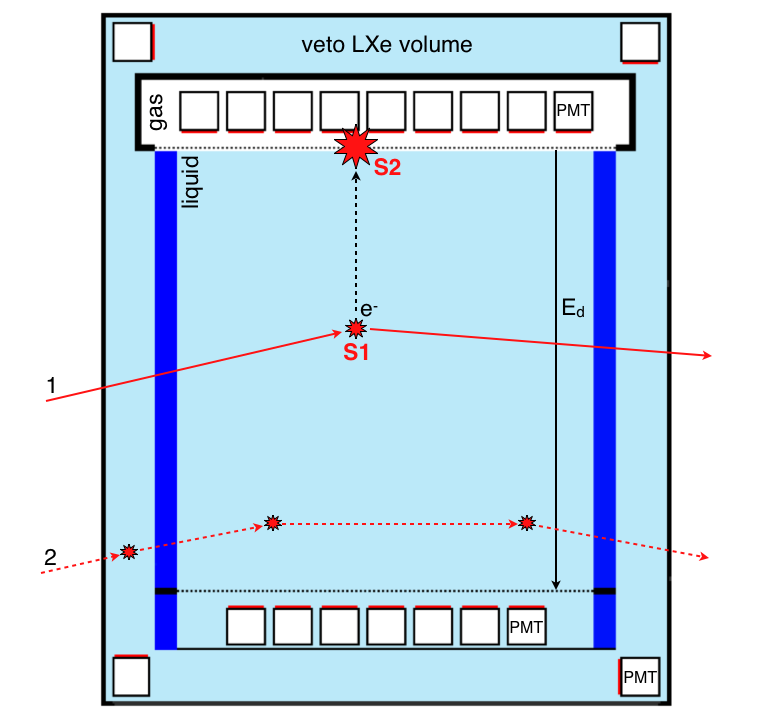
\includegraphics[width=0.495\linewidth]{plots/DetectionPrinciple/DetectionPrincipleWithLabels.png}
\caption[Particle detection principle with a double phase TPC]{Particle detection principle with a double phase TPC: 1 - valid signal event; 2 - multiple scattering event with an interaction in the liquid xenon veto volume.}
\label{figDetectionPrinciple}
%\end{figure}
\end{floatingfigure}

\begin{equation}
\label{eqScint1}
\text{Xe}^{*} + \text{Xe} \rightarrow \text{Xe}^{*}_{2},
\end{equation}
\begin{equation}
\label{eqScint2}
\text{Xe}_{2}^{*} \rightarrow 2\text{Xe} + h\nu
\end{equation}

\begin{equation}
\label{eqScint3}
\text{Xe}^{+} + \text{Xe} \rightarrow \text{Xe}^{+}_{2},
\end{equation}
\begin{equation}
\label{eqScint4}
\text{Xe}^{+}_{2} + e^{-} \rightarrow \text{Xe}^{**} + \text{Xe},
\end{equation}
\begin{equation}
\label{eqScint5}
\text{Xe}^{**} \rightarrow \text{Xe}^{*} + \text{heat},
\end{equation}
\begin{equation}
\label{eqScint6}
\text{Xe}^{*} + \text{Xe} \rightarrow \text{Xe}^{*}_{2},
\end{equation}
\begin{equation}
\label{eqScint7}
\text{Xe}^{*}_{2} \rightarrow 2\text{Xe} + h\nu
\end{equation}

The scintillation light has two components with different decay time constants (4~ns and 21~ns), corresponding to the decay of the singlet or triplet states of the excited dimer  Xe$^{*}_{2}$~\cite{SingletTriplet, SingletTriplet_dEdx}. For relativistic electrons, only one decay component with 45~ns decay time has been observed~\cite{SingletTriplet}. The pulse shapes are correlated with $dE/dx$, thus differ for particles of different type. This provides a mechanism for pulse shape discrimination (PSD). However, statistical fluctuations of the pulse shape at low energies, and fluctuations in the photon time-of-flight in the detectors of relatively large size, such as XENON100, do not allow discrimination between electronic interactions from nuclear recoils with the required precision~\cite{XenonPSD}.

%The excitation (fast) component and recombination (slow) components of the scintillation have the time dependence~\cite{SlowFastComponents}:
%\begin{equation}
%\label{eqFastSlow1}
%A_{exc} = C_{0} \cdot e^{-t/\tau_{exc}}
%\end{equation}

%\begin{equation}
%\label{eqFastSlow2}
%A_{rec} = D_{0} \cdot \frac{1 - e^{t/\tau_{exc}}}{(1+ e^{t/\tau_{rec}})^{2}}
%\end{equation}

%The time constants are . For gamma interaction, 100\% of the light is emitted in a 

Xenon atoms do not absorb their own scintillation light, because the photons originate from the decay of the excimer state. This prompt initial scintillation light (S1) is detected by photomultiplier tubes (PMTs) on the top and bottom of the target volume. 
When an electric field is applied across the liquid xenon target, some of the ionization electrons are removed from the interaction site, do not recombine and can be detected independently from the S1 light signal. The electrons created by ionization are drifted and extracted into the gas phase above the liquid xenon target, and accelerated with a high electric field, producing an electro-luminescence signal (S2)~\cite{S2} via collisions with xenon atoms, which is detected by PMT arrays above and below the target volume. 

In the standard scenario, WIMPs are expected to elastically scatter off xenon nuclei resulting in low energy nuclear recoils (NR). Neutrons with energies in $\sim$MeV range passing through the detector also produce low energy nuclear recoils, whereas $\gamma$-rays and electrons produce electronic recoils (ER). 
Because of the different $dE/dx$, the energy deposition of NR and ER results in different probability of electron-ion pairs recombination (\ref{eqScint4}), and thus different ratios of the yield of scintillation light and ionization charge. The ratio of the primary (S1) and secondary (S2) scintillation signals provides a possibility to distinguish electronic interactions (background) from nuclear recoils (signal), and to reject the electromagnetic background. Using this discrimination technique, XENON10 and XENON100 reached an ER rejection efficiency better than 99\% at $\sim$50\% NR acceptance~\cite{xe10-independent, xe100-run07}.

In a homogeneous electric field, the position in the $XY$ plane at which the proportional scintillation occurs is correlated with that of the original interaction, and leads to a clustered hit pattern on the top PMT array. This is used to reconstruct the $X$ and $Y$ coordinates of an event, as described in Chapter~\ref{chPositionReconstruction}. 
In addition, the time difference between the S1 and S2 signals provides information about the $Z$ coordinate of the interaction. The 3D position reconstruction capability allows localization and rejection of the events at the edges of the target volume, thus significantly reducing the external gamma and neutron backgrounds~(see Chapters~\ref{chERbackground} and \ref{chNRbackground}).

If a particle has deposited energy at multiple places in the target, then two or more S2 pulses are recorded in the trace. Such an event is a multiple scatter event and is rejected in the analysis since the predicted behavior of the WIMP, due to its very low scattering cross-section, would produce only single scatters~(see Section~\ref{secDataQualityCuts}).

The liquid xenon target in the XENON100 detector is surrounded from all sides by a liquid xenon layer, equipped with PMTs and acting as an active veto. Events that have a coincident signal in the veto (illustrated in Fig.~\ref{figDetectionPrinciple}) are removed from the analysis, which provides a significant reduction of background due to $\gamma$-interactions (see Section~\ref{secDetectorMaterials}).


%to exploit the self-shielding capability of liquid xenon due to its high 

